\lab{Object Oriented Programming}{Object-Oriented Programming}
\label{lab:OOP}
\objective{Illustrate the uses of OOP in programming graphical user interfaces.}

\section*{Graphical User Interfaces}

GUI's are powerful tools for creating applications that users can interact with.
PySide is a helpful library to build GUI's.
From PySide, we will use two modules, QtGui and QtCore.
QtCore has functions that will help us implement the inner workings of our GUI while QtGui will allows us to implement the graphics as well as the interface itself.
To demonstrate the main ideas behind building a GUI, we will create a simple program that displays inputted text. As you read, follow along by typing the code into a text editor and running it from your command line (type in python filename.py). Hands on experience is the best way for GUI concepts to solidify.

\begin{lstlisting}
from PySide import QtGui, QtCore

class Printer(QtGui.QWidget):
	# This class inherits from the QWidget class found in the QtGui module.
	def __init__(self):
		# Call the __init__ method from QWidget, the class Printer is sub-classed from (its "super" class).
		super(Printer, self).__init__()

\end{lstlisting}

\emph{Widgets} are what make the magic happen in GUI's.
In Qt, widgets are objects that represent various elements of a GUI.
They keep track of drawing and refreshing the graphical display of the elements, abstracting the behavior of the elements, and defining ways to interact with other widgets.
When you push a button or enter text, widgets are what notice and respond accordingly.
In our \li{Printer} we will use \li{QLineEdit} and \li{QLabel}.

\begin{lstlisting}
from PySide import QtGui, QtCore

class Printer(QtGui.QWidget):
	def __init__(self):
		super(Printer, self).__init__()
		# Call the _initUI function.
		self._initUI()
	
	def _initUI(self):
		'''Creates the widgets and tells them how to interact.'''
		
		# Create a class variable called textBar that is a QLineEdit widget.
		self.textBar = QtGui.QLineEdit()
		# Create a class variable called label that is a QLabel widget.
		self.label = QtGui.QLabel()

\end{lstlisting}

Now that we have our widgets, we need to tell them how to communicate.
Qt uses a system of \emph{signals} and \emph{slots}.
When a button is pushed or when text is entered, a widget throws a \emph{signal}.
We can specify which \emph{slot} catches the signal.
In this case, the signal being thrown is the text being entered in the text bar. We want a function that catches the signal, updates the displayed text, and clears the text bar.

\begin{lstlisting}
from PySide import QtGui, QtCore

class Printer(QtGui.QWidget):
	def __init__(self):
		super(Printer, self).__init__()
		self._initUI()

	def _initUI(self):
		self.textBar = QtGui.QLineEdit()
		self.label = QtGui.QLabel()
		
		# When return is pressed in the textBar, it sends a signal and goes into the function updateText.
        # self.textBar accesses the textBar object.
        # returnPressed defines the inputted signal.
        # connect links the signal to the method later defined in this class: updateText.
		self.textBar.returnPressed.connect(self.updateText)
	
		
	def updateText(self):
	'''Updates what text is displayed and clears the textBar'''
		self.label.setText(self.textBar.displayText())
		self.textBar.clear()

\end{lstlisting}

Next, we need to set the layout and create a function that can be called from the command line.

\begin{lstlisting}
from PySide import QtGui, QtCore
import sys

class Printer(QtGui.QWidget):
	def __init__(self):
		super(Printer, self).__init__()
		self._initUI()

	def _initUI(self):
		self.textBar = QtGui.QLineEdit()
		self.label = QtGui.QLabel()
		
		self.textBar.returnPressed.connect(self.updateText)
	
		# Create a vertical box layout.
		# This will stack all widgets added to it vertically.
		vbox = QtGui.QVBoxLayout()
		# Add textBar as a widget and display it on the first row (0) in the first column (0).
        vbox.addWidget(self.textBar, 0, 0)
		vbox.addWidget(self.label, 1, 0)
		
		# Assemble the layout.
		self.setLayout(vbox)
		# Tell the dimensions of the vbox.
		# The first two numbers indicate placement on the screen while the second two represent the dimensions.
		self.setGeometry(50, 50, 200, 200)
		self.setWindowTitle("Simple Printer")
		self.show()
	
	def updateText(self):
		self.label.setText(self.textBar.displayText())
		self.textBar.clear()
		
def main():
	# Create a QApplication.
    # Note that if you are working in IPython Notebook, you need to restart your kernel before running the program, or a RuntimeError will occur.
	app = QtGui.QApplication(sys.argv)
	# Create a Printer object.
    # Since _initUI is called in the constructor, the GUI will appear and run.
	p = Printer()
	sys.exit(app.exec_())
if __name__ == "__main__":
	main()

\end{lstlisting}

\begin{problem}
Create a simple graphical user interface that will solve the quadratic formula given the necessary parameters.
Make the GUI look similar to the one below.
\begin{figure}[H]
\centering
\begin{comment}
\begin{subfigure}[b]{.49\textwidth}
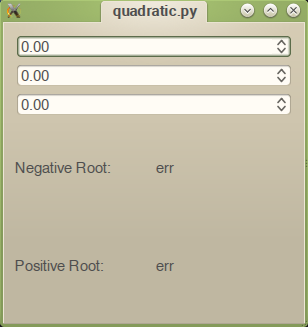
\includegraphics[width=\textwidth]{quadratic_view.png}
\end{subfigure}
\end{comment}
\begin{subfigure}[b]{.49\textwidth}
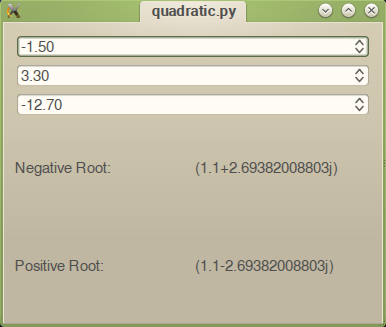
\includegraphics[width=\textwidth]{quadratic_view2.png}
\end{subfigure}
\end{figure}
The widgets that you will need are: \li{QDoubleSpinBox}, \li{QLabel}, \li{QGridLayout}, and \li{QVBoxLayout}. You may also want to import the cmath module in order to calculate complex solutions.
You can view the documentation for these classes, including all their methods and signals, at \url{http://qt-project.org/doc/qt-4.8/classes.html}
\label{prob:quadCalc}
\end{problem}


\section*{Specifications}

The following is a guideline for your solutions.

\begin{lstlisting}
import sys
from PySide import QtGui, QtCore

class People(object):
	pass
	
class ComplexNumber(object):
	pass
	
class QuadraticCalculator(QtGui.QWidget):
	pass
\end{lstlisting}